\section{Demo} \label{sec:vpake-demo}
% \mynote{Online demo and description of implementation containing\\
% * optional registration (BPR style)\\
% * server config\\
% * authentication (tSOKE style)}

To demonstrate real-world usage of the framework proposed in this Chapter we implemented a demo application that allows to set password policies, register clients, and use the registered clients to login to a demo web application.

The cryptographic password framework consists of a server and a client component.
The server is implemented in Python\footnote{\url{https://www.python.org/}} (using the bottle framework\footnote{\url{http://bottlepy.org/docs/dev/index.html}}) with a MariaDB\footnote{\url{https://mariadb.org/}} backend for data storage.
The client is implemented in JavaScript\footnote{\url{https://en.wikipedia.org/wiki/JavaScript}} as a Firefox\footnote{\url{http://firefox.com/}} extension.
This approach has the advantage of platform independence, but trades some efficiency due to the use of JavaScript.
(This could be improved using WebCrypto\footnote{\url{http://www.w3.org/TR/WebCryptoAPI/}} once it supports all necessary features.)
All code is available at \url{https://github.com/franziskuskiefer/???}.

\subsection{Registration}
The client registration has two different views that would require login for server side in a production environment, but reside on the same open website for demonstration purposes here.

\paragraph{Admin Interface}
To configure the server's password policy the admin interface (shown in Figure \ref{fig:demo-admin}) allows the web admin to define a policy expression as well as a minimum password length, prospective client passwords have to comply with.
Entered values are stored automatically for this session and used for the \ac{BPR} process.

\begin{figure}[tbph]
\centering
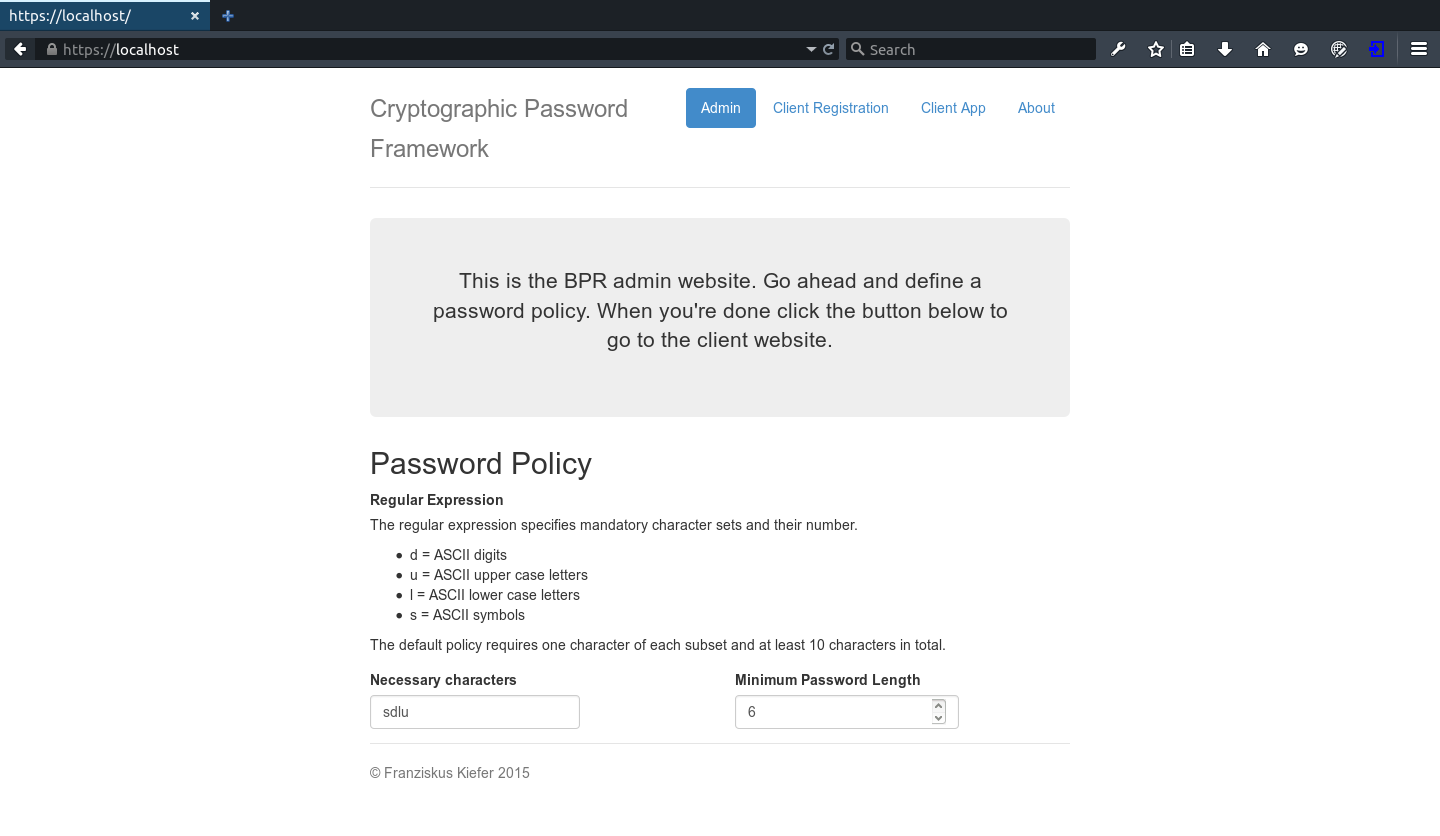
\includegraphics[width=0.98\textwidth]{Figs/demo-admin.png}
\caption{Demo --- Admin interface}\label{fig:demo-admin}
\end{figure}

\paragraph{Client Interface}
Selecting the \emph{Client Registration} link presents the user with a simple website asking the user to register a new user and password.
To this end the user has to click the registration/login button in the browser toolbar to open the registration form.
This button is only active for websites that support the \ac{BPR} registration process and provides the user with a trusted path to a trusted registration form.
Note that it is important that the registration form is trusted and \emph{not} provided by the server as the server is not trusted with secure handling of the client password.
After clicking ``Register Now'' the extension performs the \ac{BPR} protocol from Section \ref{sec:bpr} with the server.
The JavaScript implementation makes use of cryptographic libraries\footnote{\url{http://www-cs-students.stanford.edu/~tjw/jsbn/}, \url{https://github.com/bitwiseshiftleft/sjcl}}), while the server uses the Charm library by \citet{charm13}.

\begin{figure}[tbph]
\centering
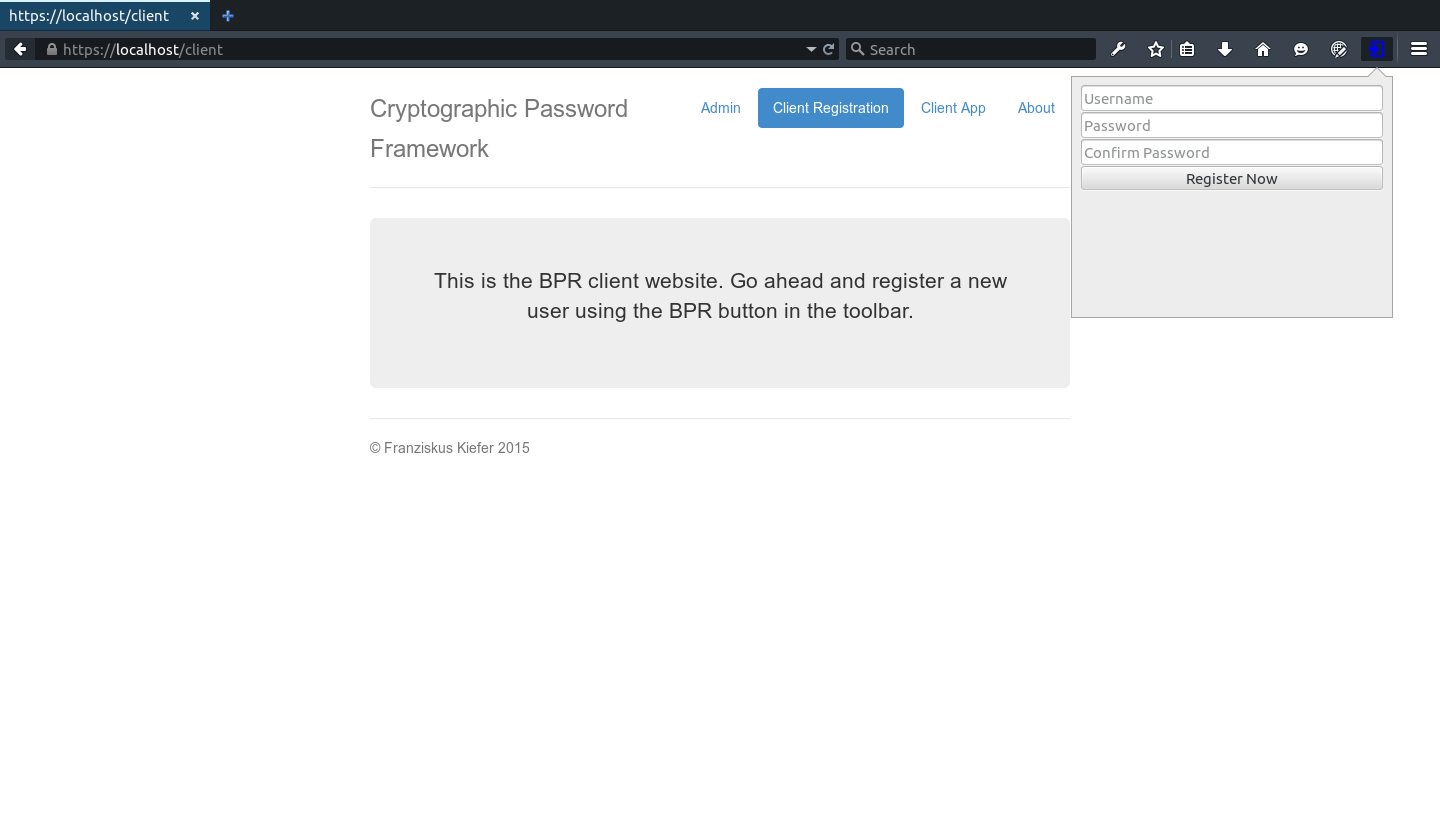
\includegraphics[width=0.98\textwidth]{Figs/demo-register-popup.png}
\caption{Demo --- Client Registration interface}\label{fig:demo-register}
\end{figure}

\subsection{Login}
Clicking on the ``Client App'' link provides the user with a simple website asking the user to log into the application using the registration/login button in the browser toolbar.
Similar to the registration process, the user is presented with a trusted login form.
After entering user name and password, and clicking ``Login'', the extension performs the tSoke protocol with the server.
As discussed before, tSoke is a \ac{VPAKE} protocol that additionally uses a tag to make it usable in the \ac{PACCE} setting.
Thereby, client and server perform a \ac{PACCE} protocol, which hands the session over to the client application when done.

\begin{figure}[tbph]
\centering
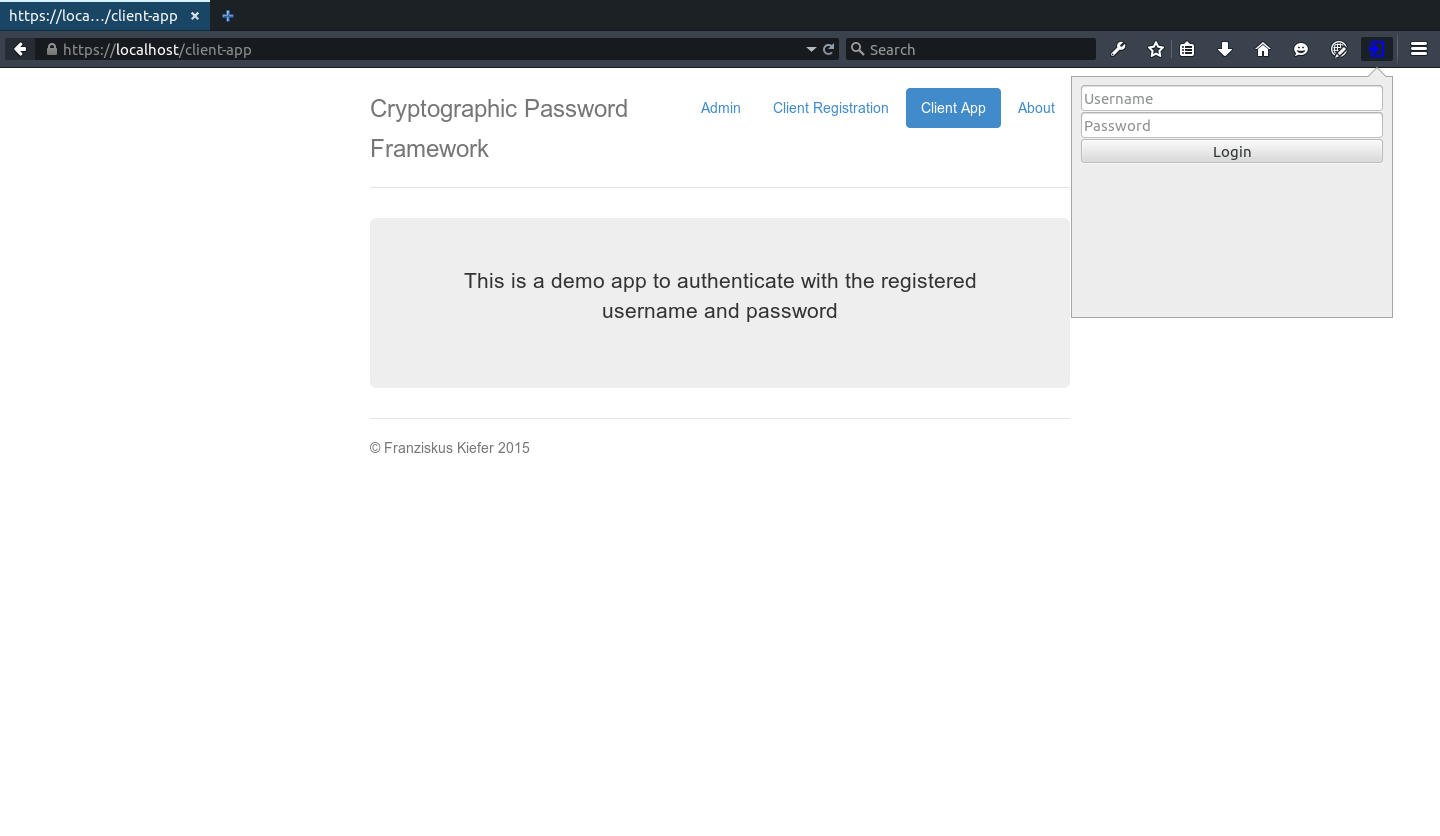
\includegraphics[width=0.98\textwidth]{Figs/demo-login-popup.png}
\caption{Demo --- Client Login interface}\label{fig:demo-login}
\end{figure}

\subsection{Demo Application}
The client demo application, a simple to-do application, is depicted in Figure \ref{fig:demo-app}.
It is an independent component and embedded in the framework website as an iframe.
It uses NodeJS\footnote{\url{https://nodejs.org/}} as RESTful\footnote{\url{https://en.wikipedia.org/wiki/Representational_state_transfer}} server, MongoDB\footnote{\url{https://www.mongodb.org/}} for storage, and jade\footnote{\url{http://jade-lang.com/}} as template engine.

\begin{figure}[tbph]
\centering
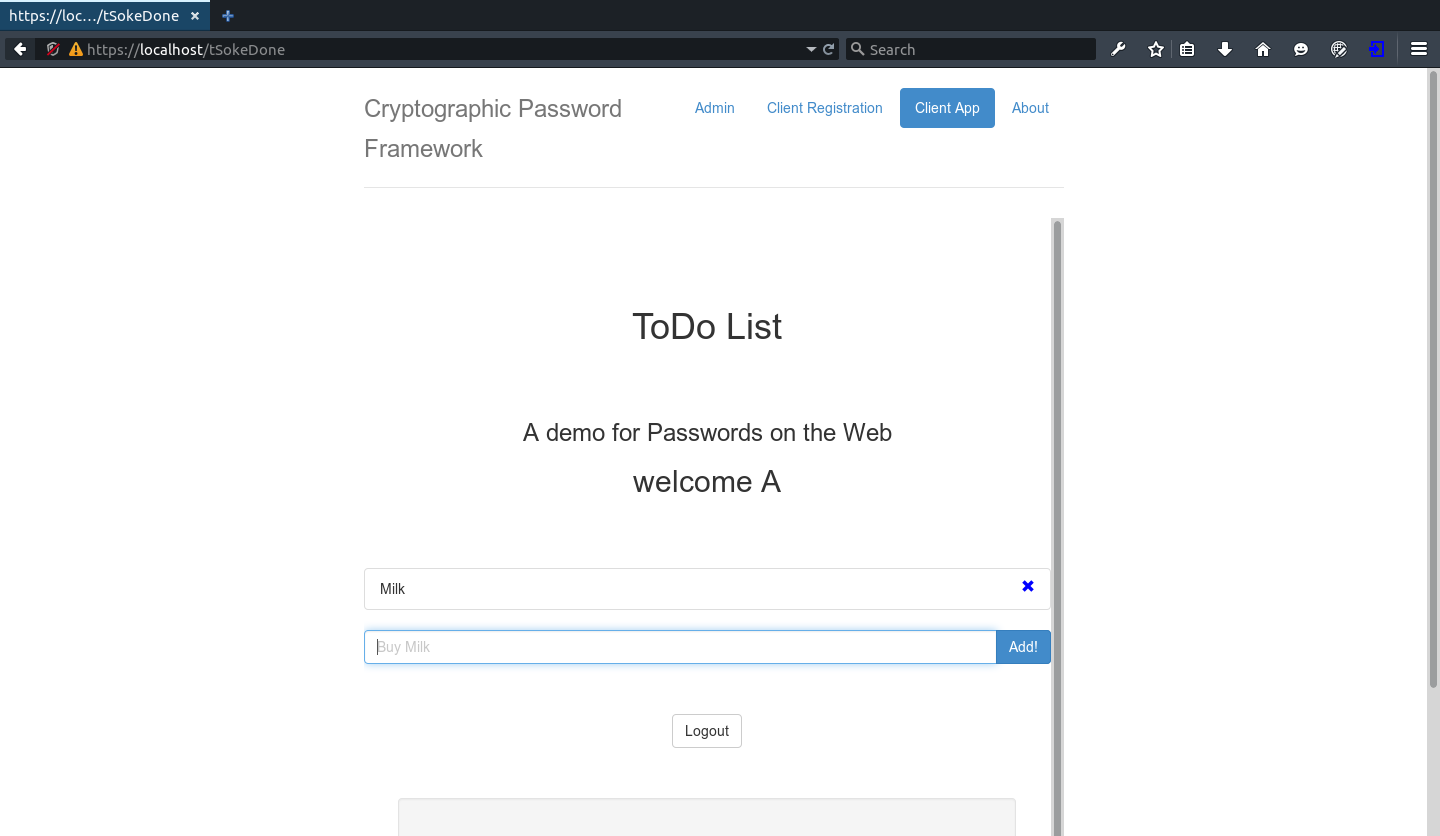
\includegraphics[width=0.98\textwidth]{Figs/demo-app.png}
\caption{Demo --- Client Application interface}\label{fig:demo-app}
\end{figure}
